% !TEX root = ../prospector.tex

\section{Motivation}

\subsection{Machine Learning for Predictive Modeling}

Data scientists often use machine learning to create predictive models based on known properties of  training data, which acts as the ground truth. 
%Predictive modeling is a machine learning discipline that uses observed data to predict unobserved outcomes.
%Often classification is used that instead of having a numeric outcome like risk has a few categories.
%Numeric outcomes can always be converted into categories.
%For example risk can be categorized into low, medium, and high risk.
Machine learning algorithms typically work in two phases: the training phase and the prediction phase.
In the training phase, parameters of the model are
learned using training data.
%In the training phase, outcomes from training data are used to verify the quality of prediction and make changes to internal values of the model until a local maximum is reached.
% Typically unstructured data is converted into feature vectors to be usable with common machine learning algorithms.
The prediction phase then computes predictions using the trained model. % The model does not change in this phase anymore.
Below, we describe several machine learning algorithms that are commonly used and also utilized in the case study.

A decision tree is one such algorithm, which is a tree whose nodes are rules that decide how to proceed down the branches of the tree, according to the range of values for a specific feature.  The decision making starts at the root of the tree and leaves carry the prediction results. Decision trees are popular in machine learning as they allow data scientists to model arbitrary functions.
However, the more nodes a tree has, the harder it is to understand the reasoning behind outcomes.
Logistic regression is another popular algorithm that is easier to understand, as features can only positively or negative influence the prediction, and the rate of influence is fixed.  This is achieved by defining a hyper-plane in the feature vector space, where the outcome of the prediction depends on how close to and on which side of the hyper-plane an instance is.

% Each feature contributes linearly to the outcome.
% So a low value of a feature leads to a low outcome and a high value to a high outcome or a low value leads to a
% high outcome and a high value to a low outcome.
% Each feature is assigned one weight that determines how rapid changes in the value change the outcome.

Another popular algorithm is random forests, which combine the output of multiple decision trees.
A random forest is an example of an ensemble model, which combines the output of several weak machine learning models to yield an overall better result with less bias and variance than a single strong model.
% Random forest is an example of a boosting model, which works under the assumption that combining the output of several weak machine learning models yield an overall better result than a single strong model.
However, this makes ensemble models less interpretable since each weak model has only a small influence on the outcome.
% Random forests are boosting models consisting of decision trees that are built using randomized thresholds that are improved during the training phase.  Randomization is necessary since otherwise all trees would be identical.


\subsection{Predictive Modeling in Health Care}

In order to make our contributions concrete, we utilize a motivating scenario that emerged from our case study.  The case study involves a team of five data scientists interested in using predictive modeling on a longitudinal database of electronic medical records. The research team has a background in health care analytics and their database contains 4,000 patients from a major hospital in the United States. The team is interested in building a predictive model to predict if a patient is at risk of developing Diabetes, a chronic disease of high blood sugar levels that may cause serious health complications.

% !TEX root = ../prospector.tex

\begin{figure}
\centering
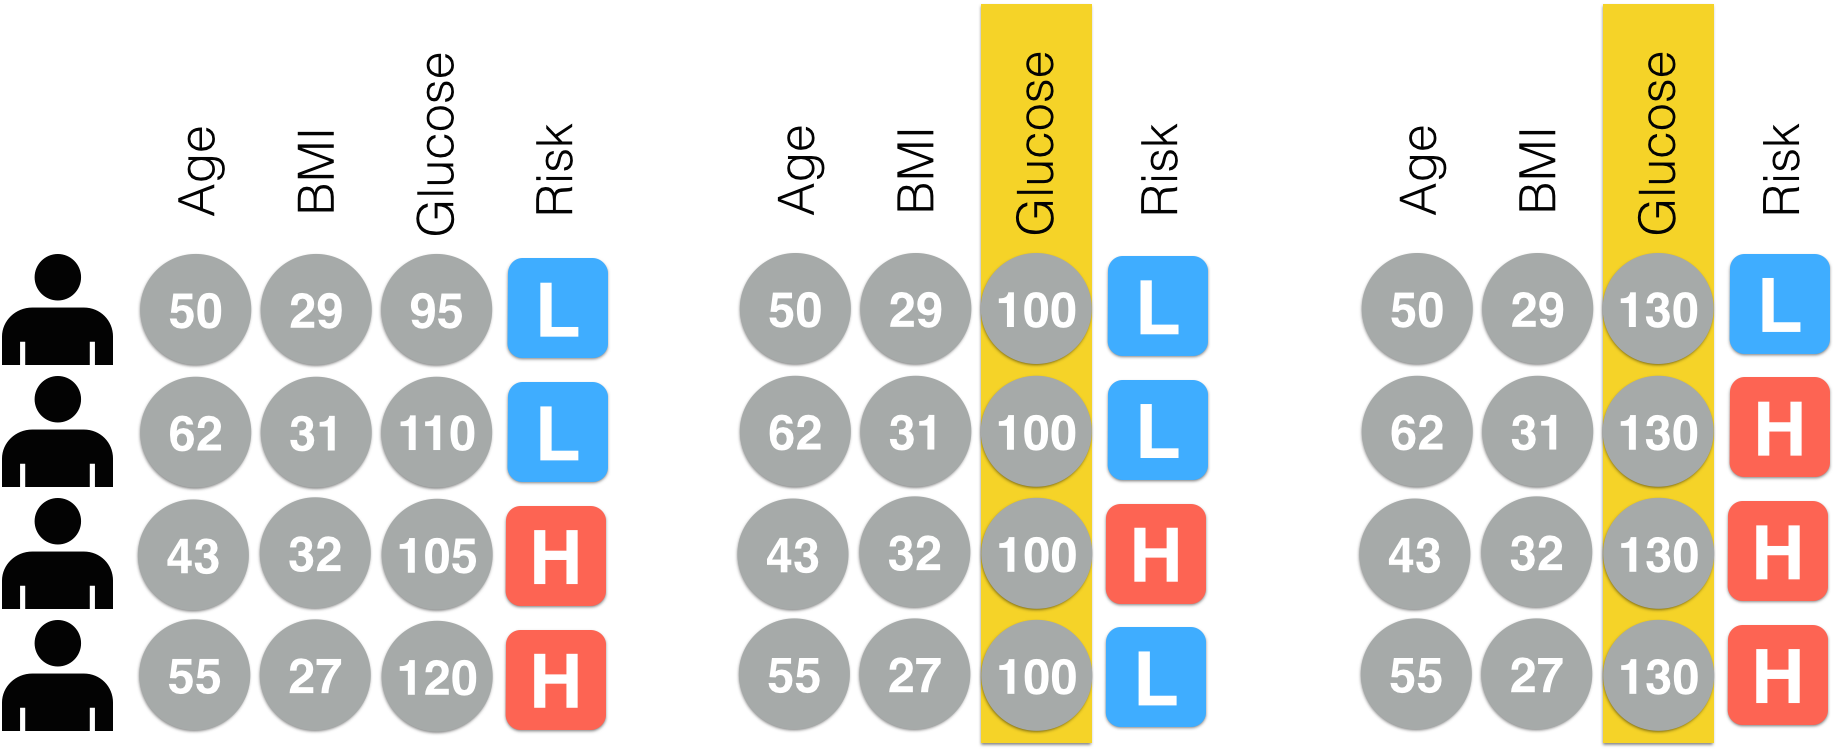
\includegraphics[width=0.90\linewidth]{prospector/partial-dependence-explanation} % 0.95
\caption{
An illustration of how partial dependence is computed for the feature ``Glucose".  On the left are four patients' original feature values.  In the middle, the ``Glucose" values are all changed to 100, and the corresponding predictions change.  Similarly, on the right, the ``Glucose" values are all changed to 130, and again the risks are different.  This demonstrates the impact of the ``Glucose'' feature on risk prediction.
% The plotted value in a Partial Dependence plot is the average of the
% ``Risk" probability values.
}
\label{figs:pdexplain}
\end{figure}

The team of data scientists manages to develop a highly accurate predictive model for detecting patients at high risk of developing Diabetes.  They determine its effectiveness by measuring the common metrics used by predictive models (e.g., accuracy and AUC scores \cite{kuhn2013applied}).  They also followed the best practices of building predictive models.  They worked with clinical researchers to properly define cohorts of patients with Diabetes (cases) and matched patients without Diabetes (controls) by thoroughly searching through the electronic medical records.  They constructed features based on lab tests, diagnosis codes, procedures, demographics, and patient conditions from the records.  They used cross-validation to ensure their models were robust.  They used a variety of state-of-the-art feature selection methods to utilize the most informative features in the model while keeping it as generalizable as possible.  And they used a variety of effective classifiers to do the training and evaluation.  After trying various combinations of these techniques, the model with the highest accuracy metrics was selected and presented to the appropriate stakeholders at the health care institution.

Their stakeholders were impressed by the high accuracy scores of the model.  But when they asked the data scientists for more information about what was inside of the model, the reports only described the top features of the model and their associated ``importance" weights.  The stakeholders recognized many of the feature names, and it appeared to make clinical sense.  However, there were also some surprising ones that led to intellectual discussions.  But the stakeholders demanded to know more.  They wanted a clearer sense of how certain features impacted the prediction.  Furthermore, they wanted to understand how the values associated with the features (\eg, the results associated with lab tests) impacted the prediction.  They also were curious to interact with the model to test hypotheses about how the model would react to hypothetical patients of interest.  When confronted with these questions, the data scientists shrugged.  In the data scientist's defense, it is difficult to summarize and interpret complex models and there are few tools and techniques available to address the stakeholders' requests.  So now the stakeholders are faced with a hard decision:  do they deploy a predictive model in their institution that appears to have high accuracy but is also somewhat of a black-box?

Although this scenario is motivated by our case study, our other projects and interviews suggest these are not atypical requirements.  Our work is motivated to support the development of more comprehensible predictive models. 

\subsection{Partial Dependence}

% !TEX root = ../prospector.tex

\begin{figure}[t]
\centering
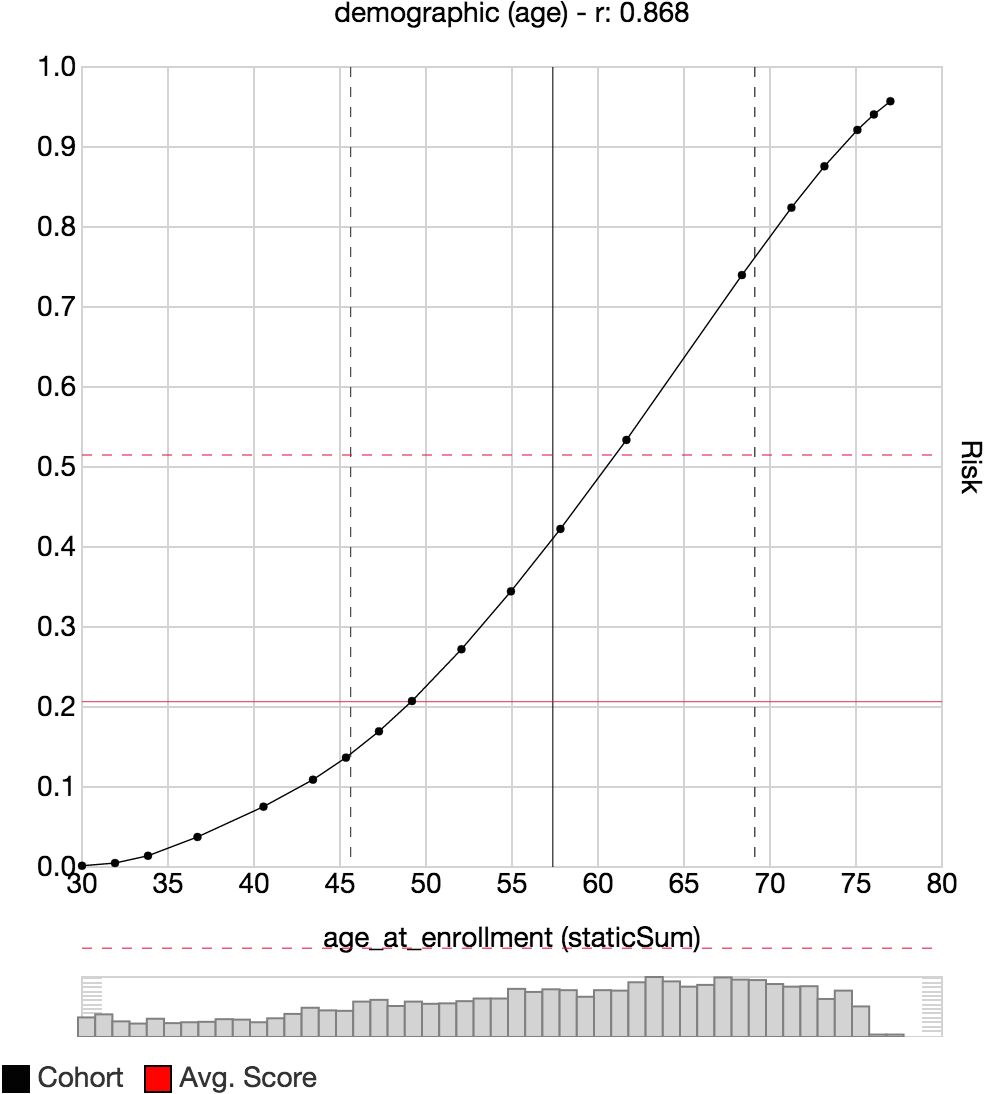
\includegraphics[width=0.55\linewidth]{prospector/pdp_reg} % 0.7
\caption[Partial dependence plots.]{
Partial dependence plots. The black curve shows the average predicted risk
(probability of a certain outcome) if for all rows in the data the value of this
feature was the given value of the horizontal axis.
The red line shows the average predicted risk for the original data.
The vertical line shows the mean of the observed values and the histogram below the plot
shows the distribution of observed values.
Dotted lines show the range of one standard deviation around the mean values.
}
\label{figs:pdp}
\end{figure}

The most widely used technique to understand the relationship between a feature and a prediction is by computing partial dependence \cite{friedman2001,hastie2001}.
The idea of partial dependence plots is to treat predictive models as a black-box and observe how changes in the input affect prediction outcomes.
When inspecting only the partial dependence of one input feature at a time, Formula (\ref{eq:pdp}) can be used to compute a partial dependence plot.

\begin{equation}
pdp_f(v) = \frac{1}{N} \sum_i^N pred(x_i) \;\text{with}\; x_{if} = v
\label{eq:pdp}
\end{equation}

$N$ is the number of rows in the input matrix $x$,
$pred$ is the prediction function that takes one input row, a feature vector, and returns an outcome probability,
and $f$ is the feature used to compute the partial dependence plot.
The formula computes the average outcome over all input rows while changing the value of feature $f$ to the
input value $v$ for each row $x_i$. The original input data is kept fixed. This allows for observing the influence of $f$
on the predicted probabilities.

In order to make this function more concrete, consider the illustrative example in Figure~\ref{figs:pdexplain}, where each input row is a patient, and each column is a feature.  The last column represents the output of the predictive model that predicts if a patient is at low-risk or high-risk for developing Diabetes.  In Figure~\ref{figs:pdexplain}a, the patients' original feature values (age, BMI (Body Mass Index, a standard way to quantify obesity), and glucose level (a standard way to determine Diabetes)) are shown.  If one wants to examine the impact of the glucose feature on the prediction, partial dependence can be applied by keeping all of the other features (age, BMI) as they were, but fixing glucose to a set of fixed values to see how that feature impacts the prediction.  For example, in Figure~\ref{figs:pdexplain}b, the glucose values (highlighted in yellow) are fixed to 100, which yields predictions of only 1 patient being high risk, instead of the original 2.  Conversely, in Figure~\ref{figs:pdexplain}c, glucose is fixed to 180, and 3 patients are predicted to have high risk.  Thus, there appears to be partial dependence of glucose on the prediction.  

Partial dependence is typically visualized as a partial dependence plot, as shown in Figure~\ref{figs:pdp}, which is a line graph that plots the fixed values of the target feature on the x-axis, and the corresponding predicted risk (\ie, probability of a certain outcome) on the y-axis.  

